
\section{Tables and graphs}

%Should any of the generic/abstract graph drawing should be here.  It can certainly move to an appendix instead, and then rewrite this section to cut quickly to the graph.

%% SU -- what should the standard number of boxes across and up be, for the purpose of this text.  Is there a standard graph paper template to use?
%GraphPaper.png is 24 across (same as this graph, by the way) and 16 up.

% In the DYK need a "ask your instructor" about what sorts of graphing technology are available.

Lung cancer, chronic bronchitis, bad breath, stains on your clothes, and the expense.  These are just a few of the consequences of smoking cigarettes. With what we know now about the dangers of smoking, are people smoking more or less than they were ten years ago, fifty years ago, or even one hundred years ago?  

Reality is, we don't have information on each individual person's smoking rate, so we can't answer this question exactly.  We do have information on the total number of cigarettes sold each year.  So maybe we should look at that total. Uh oh, that isn't going to work.  There are way more people now than there were fifty or a hundred years ago.  So, even if the same percentage of people smoke, and even if they each smoke the same amount as their predecessors did, we would have a much bigger number of cigarettes smoked now just because there are more people now.  

Turns out a reasonable measure is to compare the number of cigarettes smoked per year \emph{per person}.  By taking into account the number of people we will be able to see whether people are smoking more or less, on average. That's what we want.  

Here are some representative years from the Center for Disease Control for the United States. 
%http://www.cdc.gov/tobacco/data_statistics/tables/economics/consumption/  Retrieved July 5, 2012
 The smoking rate is the average cigarettes per year per person.  (Here ``person'' only includes adults.)
\begin{center}
\begin{tabular} {|c| |c|c|c|c|c|c|c|c|c|c|} \hline
Year & 1900 & 1915 & 1930 & 1940 & 1950 & 1965 & 1975 & 1990 & 2000 & 2006 \\ \hline
Smoking rate & 54 & 285 & \text{1,485}& \text{1,976} & \text{3,552} &  \text{4,258} &  \text{4,122} &  \text{2,834} &  \text{2,049} &  \text{1,619} \\ \hline
\end{tabular}
\end{center}
\bigskip 

To make sense of these numbers, suppose there are five friends.  Three don't smoke at all, so that is 0 cigarettes in a year.  Another smokes only occasionally, maybe 100 cigarettes a year.  The fifth smokes ``a pack a day,''  which adds up to \text{7,300} cigarettes in a year because
$$\frac{1\text{ pack}}{\text{day}} \ast \frac{20\text{ cigarettes}}{\text{pack}} 
\ast \frac{365 \text{ days}}{\text{year}} 
=20 \times 365
= \frac{\text{7,300 cigarettes}}{\text{year}} $$
(Not sure about this calculation?  Not to worry.  More about unit conversions in \S1.4.) % SU ref section \#
These five people smoke a total of $$0+0+0+100+\text{7,300}=\text{7,400 cigarettes per year}$$
so when we divide by the number of people we get
$$\frac{\text{7,400 cigarettes per year}}{5 \text{ people}} = \text{7,400} \div 5 = \text{1,480 cigarettes per year per person}$$
This group is fairly typical for the United States in 2012.  They smoke less than the average of \text{1,619} cigarettes per year per person for 2006 (the last year the CDC published the data). 

We can tell a lot of information from this table.  For example, what was the smoking rate in 1964, and how does that compare to 2006?  The answers appears in the table, a whopping \text{3,552} cigarettes per person in 1964 and \text{1,619} cigarettes per person in 2006.

When did the consumption first pass \text{3,000}?  That answer does not appear in the table, but we can use the information in the table to make a good guess.  In 1940, there were an average of \text{1,976} cigarettes per person per year and by 1950, there were \text{3,552}.  Somewhere between 1940 and 1950 the number first climbed above \text{3,000}.  More specifically, the number we're looking for (\text{3,000}) is a lot closer to the 1950 figure (\text{3,552}) than to the 1940 figure (\text{1,976}).  So, it would be reasonable to guess close to 1950.  I'd say 1947.  Of course, you might guess 1946 or 1948, or even 1949 and those would be good guesses too.  

When did the consumption drop below \text{3,000} again?  This answer also does not appear in the table, but falls somewhere between 1975 when consumption was \text{4,122} and 1990 when consumption was  \text{2,834} .  Here I'd guess just before 1990, say in 1989.   

What's changing are the number of cigarettes smoked per person per year and the year.  Those are our variables.  The smoking rate is a function of year, and it's what we care about, so it's the dependent variable.  Time, as measured in years, is the independent variable.   
\begin{center}
\begin{tabular} {l}
$S=$ smoking rate (cigarettes per year per person) $\sim$ dep \\
$Y= $ year (years since 1900) $\sim$ indep \\ 
\end{tabular}
\end{center}
Quick note on how we deal with actual years.  Since the year 0 doesn't make sense in this problem, it is convenient to measure time in years since 1900. Officially we should rewrite our table as:

\begin{center}
\begin{tabular} {|c| |c|c|c|c|c|c|c|c|c|c|} \hline
$Y$ & 0 & 15 & 30 & 40 & 50 & 65 & 75 & 90 & 100 & 106 \\ \hline
$S$ & 54 & 285 & \text{1,485}& \text{1,976} & \text{3,552} &  \text{4,258} &  \text{4,122} &  \text{2,834} &  \text{2,049} &  \text{1,619} \\ \hline
\end{tabular}
\end{center}

Notice where the variable names are listed in the table. In a horizontal format like this table, the independent variable ($Y$) is in the top row, with the dependent variable ($S$) is in the bottom row.  If you want to write your table in a vertical format, that's okay too.  Just put the independent variable in the left column, with the dependent variable in the right column. It might help to remember that the independent variable goes first (either top or left) and the dependent variable follows (either bottom or right).  

 \begin{center}
 \begin{figure} [h]
\begin{minipage}{3.5in} 
Horizontal table format:

\bigskip

\begin{tabular} {|c| |c|c|c|c|} \hline
indep & \hspace{.5in} & \hspace{.5in} & \hspace{.5in} &\hspace{.5in}  \\ \hline
dep & & & & \\ \hline
\end{tabular}
\vspace{.6in}  % VSPACE
\end{minipage} 
\begin{minipage}{2.5 in} 
Vertical table format:

\bigskip

\begin{tabular} {|c| c|} \hline
\hspace{.05in}  indep \hspace{.05in} & \hspace{.1in} dep\hspace{.1in} ~  \\ \hline \hline
&  \\ \hline
& \\ \hline
& \\ \hline
& \\ \hline
\end{tabular}
\end{minipage} 
\end{figure}
\end{center}
\vspace{-.3in}  % VSPACE

Where the variables go in a table is not something you can figure out.  It's a \textbf{convention} -- a custom, practice, or standard used within the mathematical community.  Though based on reason, it often involves some arbitrary choice, which is why we can't figure it out.  So, whenever some practice is introduced to you as a ``convention'', you need to memorize it.  
%Might be time to start a \textbf{don't  forget list}.  First up: where dependent and independent variables go in a table.
 
Tables are useful because they contain specific numbers, but it can be difficult to guess or see general trends.  For that, a picture is worth a thousand words -- or numbers, in this case.   By picture we mean the graph of the function.  

Throughout this text, we draw graphs by hand.  On graph paper.  Seriously.  You might wonder why we do that  when graphing calculators, spreadsheet programs, graphing ``apps,'' or computer algebra systems all can draw graphs for us.  The answer is we want to understand graphs better.  I promise -- drawing them by hand will help you do that.  Different folks have different opinions on the importance of graphing by hand, so be sure to ask your instructor what you are expected to do.  Even if you're allowed to use some type of graphing technology, I strongly encourage you to practice drawing graphs by hand as well.

There is a standard set up for a graph.
\begin{center}
\scalebox {.8} {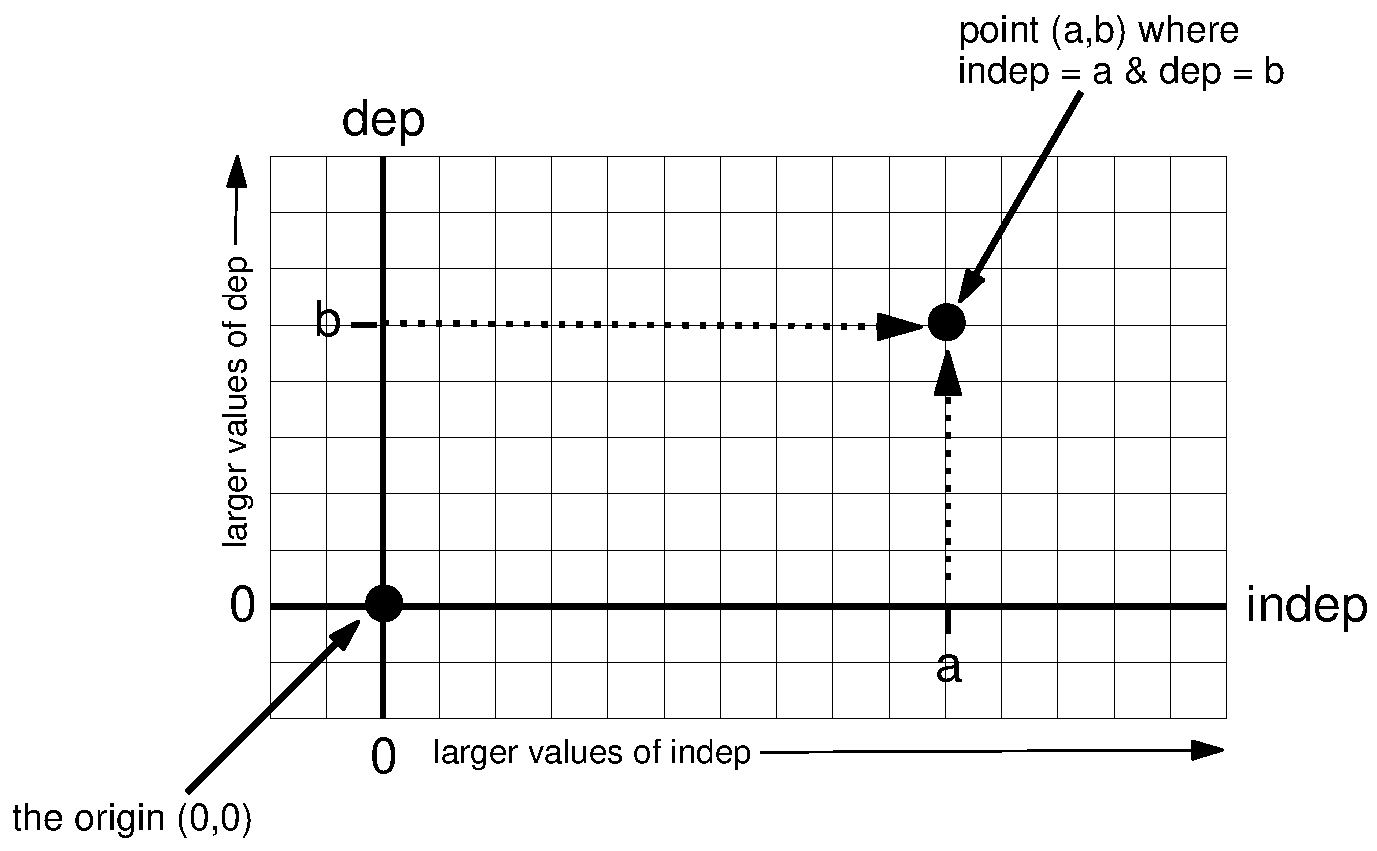
\includegraphics [width = 6in] {GraphLabelAxes.pdf}}
\end{center}
The graph is based on a horizontal line and vertical line, called the \textbf{axes}.  Where they cross is a point called the \textbf{origin}.  It represents where each variable is 0.  By convention, the independent variable is measured along the horizontal axis, with larger values progressing to the right of the origin, and negatives to the left.  Similarly, the dependent variable is measured along the vertical axis, with larger values progressing up from the origin, and negatives down.  Each gridline counts the same number, called the \textbf{scale}, but the scale for the vertical may be different from the scale for the horizontal.  Each pair of values of the independent and dependent variable from our table correspond to a point on our graph.  

In the graph of smoking rates, the independent variable is $Y$, the year, so that goes on the horizontal axis for our graph.  Our dependent variable is $S$, the smoking rate, so that goes on the vertical axis.  For the scale, it works nicely to count by 10 years and count by 500s for the smoking rate. 

There's a certain amount of guess and check involved in figuring out a good scale for each axis.  As a general rule of thumb we would like the graph to be as large as possible so we can see all of its features clearly.  But, not so big that it runs off the graph paper.  What matters is that the gridlines are evenly scaled and that they can handle large enough numbers.  Speaking of which, it's a good idea to leave a little room to extend the graph a little further than the information we have in the table, in case we get curious about values beyond what we have already. 

With realistic numbers it's normal to have numbers in the table that are not exactly where the gridlines are. It is very helpful to count by round numbers (2s, 5s, 10s, etc.) because it makes guessing in between easier.  Easier for you drawing the graph.  Easier for someone reading your graph.  

\begin{center}
\scalebox {.9} {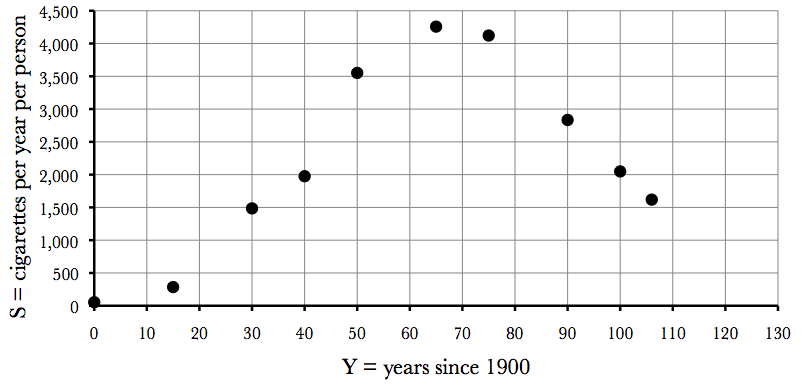
\includegraphics [width = 6in] {CigScatter3.png}}
\end{center}

To plot each point, we start at the origin and move right to that $Y$-value, and then up to that $S$-value.  When a value doesn't land exactly on a grid mark, we have to guess in between.  For example, in 1900, when $Y=0$ so we don't move right at all, just up to $S=54$.  The first labeled gridline on our graph is 500.  Where's 54?  It's  between 0 and 500, very close to 0.  Our point is just a tiny bit above the origin.  In 1915 we have $Y=15$. Our labeled gridlines are for 10 and 20, so 15 must land halfway in between.  The smoking rate to 285, which is around halfway between 0 and 500.  Etc.

What we have so far is a \textbf{scatter plot} of points.  Can you see why it's called that?  Anyway, our whole goal here was to be able to understand smoking rates better by having a graph.  You may already begin to see a curve suggested by the points. Time to draw it in.  I don't mean drawing a line between each pair of points, like you do in the children's game ``connect the dots.''  That isn't quite right.  It was probably more of a continuous trend and so the graph should be smoother.  
% SU need to fix gridlines here, and axis labels
\begin{center}
\scalebox {.9} {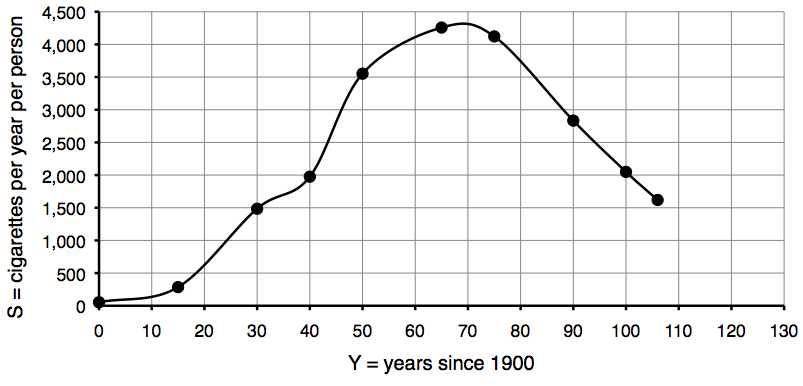
\includegraphics [width = 6in] {CigCurve.png}}
\end{center}

When we draw in this smooth curve for the graph, what we are really doing is making a whole lot of guesses all at once.  For example, from the table we guessed that the smoking rate passed  \text{3,000} in around 1947, and dropped back to that level in around 1989.  What does the graph show?  If we look where the horizontal gridline for \text{3,000} crosses our graph, it crosses in two places.  First, between the vertical gridlines for 40 and 50, and perhaps slightly closer to 50.  I'd say $Y \approx 47$, in the year 1947.  Sure.  The second time is between the gridlines for 80 and 90, much closer to 90.  Looks like $Y \approx 88$, in the year 1988. We guessed 1989.  Close enough.

Don't forget that when we drew in that curve it was really just a guess.  We're sure about the points we plotted, but we're only guessing about where to draw the curve in.  That means we're not sure about the other points.  If we knew a lot more points we could have a more accurate graph. 

Turns out  more data is available from the CDC.  The full table of data from the CDC shows that consumption first topped \text{3,000} as early as 1944.  Here's an example where the history tells you more than the mathematics as cigarette consumption rose sharply during World War II.  Our guess about 1988 or 1989 was spot on.  Look at how the graph from the full data compares to our guess.  

\begin{center}
\scalebox {1.1} {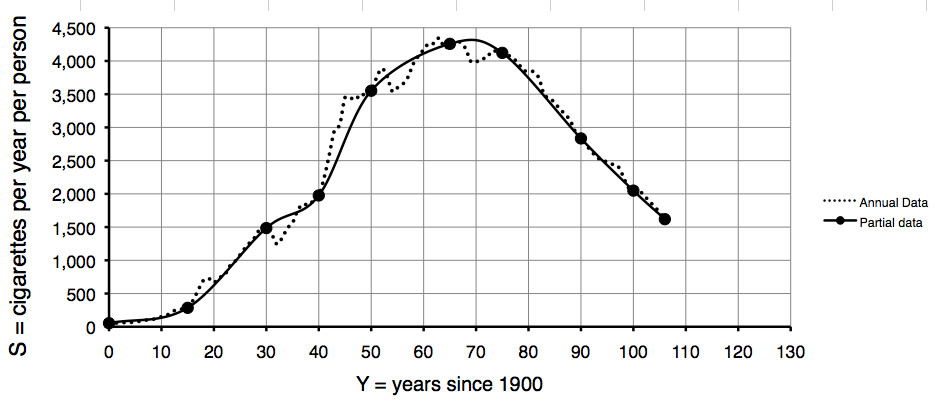
\includegraphics [width = 6in] {CigCompare.png}}
\end{center}



%\newpage

%%\section{Tables and graphs}

\begin{center}
\line(1,0){300} %\line(1,0){250}
\end{center}

\section*{Homework}

\noindent \textbf{Start by doing Practice exercises \#1-4 in the workbook.}

\bigskip

\noindent \textbf{Do you know \ldots}

\begin{itemize}
\item Where the independent and dependent variables appear in a table and in a graph? 
\item How to guess values from a table or from a graph? 
\item How to make a graph from a table?
\item Why we start each axis at 0? 
\item What we mean by scaling an axis evenly? 
\item How to make a table and then a graph from a story? 
\item Why we draw in a smooth line or curve connecting the points? 
\item What type of graphing technology, if any, you're allowed to use?  \emph{Ask your instructor.}
\item[~] \textbf{If you're not sure, work the rest of exercises and then return to these questions.  Or, ask your instructor or a classmate for help.}
\end{itemize}

\subsection*{Exercises} 

\begin{enumerate} 
\setcounter{enumi}{4}

\item The table lists estimates of Earth's population, in billions, for select years since 1800.   
\begin{center}
\begin{tabular} {|l ||c |c |c |c |c |c |c |} \hline
Year & 1800 & 1850 & 1900 & 1950 & 1970 & 1990 & 2000 \\ \hline
Population & 0.98 & 1.26 & 1.65 & 2.52 & 3.70 & 5.27 & 6.06  \\ \hline
\end{tabular}
\end{center}
\hfill \begin{footnotesize} Source:  ``The World at Six Billion'' United Nations report\end{footnotesize}
%http://www.un.org/esa/population/publications/sixbillion/sixbilpart1.pdf

 \hfill \emph{Story also appears in 1.3 Exercises}
 
Use the table to find or reasonably guess the answers to the following questions.
\begin{enumerate}
\item What was the population of Earth in 1850?
\item What do you think the population of Earth was in 1860?
\item What do you think the population of Earth was in 1960?
\item In what year do you think the population of Earth first exceeded 2 billion?
\item In what year do you think the population of the world will exceed 7 billion?
\item Identify the variables, including units and dependence.
%\item Draw a detailed graph illustrating the dependence based on the points given in the table.  SAVE GRAPH FOR NEXT SECTION
\end{enumerate}  

\item Your local truck rental agency lists what it costs to rent a truck (for one day) based on the number of miles you drive the truck.
\begin{center}
\begin{tabular} {|l ||c |c|c|c|} \hline
Distance driven (miles) & 50 & 100 & 150 & 200 \\ \hline
Rental cost (\$) & 37.50 & 55.00 & 72.50 & 90.00 \\ \hline
\end{tabular}
\end{center}
 \hfill \emph{Story also appears in 1.3 and 4.4 Exercises}
 
Use the table to find or reasonably guess the answers to the following questions.
\begin{enumerate}
\item How much does it cost to rent a truck if you drive it 100 miles?
\item How many miles did you drive a truck costing \$90.00 to rent?
\item If you rent a truck and drive it 75 miles, how much do you think it will cost?
\item If you rent a truck and drive it 10 miles, how much do you think it will cost?
\item If you rent a truck and it costs \$60.00, about how many miles was it driven?
\item Identify the variables, including units, realistic domain, and dependence.
\item Draw a detailed graph illustrating the dependence based on the points given in the table.  Be sure your axes are labeled and evenly scaled.  Sketch in a smooth curve connecting the points.
\item Use your graph to check your answers to the questions.  Modify,  if necessary.
\end{enumerate}  

\item The temperature was 40$^\circ$F at noon yesterday downtown Minneapolis but it dropped 3$^\circ$F an hour in the afternoon.    \hfill \emph{Story also appears in 1.1 and 4.1 Exercises}
\begin{enumerate}
\item Make a table of reasonable values.
\item Draw a graph illustrating the dependence.  Count time in hours after noon.
\item According to your table and graph, when did the temperature drop below freezing (32$^\circ$F)?
\item According to your graph, when did the temperature drop below 0$^\circ$F.  Does that seem realistic?  \emph{Here in the midwest there are no oceans or mountains to moderate large temperature changes.}
\end{enumerate} 

\item Mrs.\ Nystrom's Social Security benefit was \$746.17/month when she retired from teaching in 2009. She had taught in elementary school since I was a girl.   Benefits have increased by 4\% per year.  \hfill \emph{Story also appears in 1.1 and 5.1 Exercises}
\begin{enumerate}
\item Make a table of reasonable values using $N$ for Mrs.\ Nystrom's benefits (in dollars) and $Y$ for time (in years since 2009).  
\item Draw a graph illustrating the dependence.  Scale your graph to show up through the year 2020 and \$1,200.
\item According to your table and graph, when did her benefit pass \$900/month?
\item If you extend your graph to 2020, what would you estimate Mrs.\ Nystrom's benefit will be then, assuming these increases continue?
\end{enumerate}  

\item The table adapted from shows the ``heat index'' as a function of humidity at an air temperature of 88$^\circ$F. With up to about 40\% humidity, 88$^\circ$F feels like it's 88$^\circ$F. But if the humidity rises to 60\%, then it feels like it is 95$^\circ$F;  that is, the heat index is 95$^\circ$F.  
\begin{center}
\begin{tabular} {|l| |c|c|c|c|c|c|} \hline
Humidity (\%)  & 50 & 60 & 70 & 85 & 90 & 95 \\ \hline
Heat index ($^\circ$F)  & 91 & 95 & 100 & 110 & 113 & 117 \\ \hline
\end{tabular}
\end{center}
\hfill \begin{footnotesize} Source:  National Oceanic and Atmospheric Administration  \end{footnotesize}
% http://www.crh.noaa.gov

All of the following questions refer to situations when the air temperature is 88$^\circ$F.
\begin{enumerate}
\item What is the heat index when the humidity level is 70\%?
\item At what humidity level does it feel more like 98$^\circ$F?
\item Heat exhaustion is likely to occur when the heat index reaches 105$^\circ$F.  At what humidity level will heat exhaustion likely occur?
\item The heat index is considered danger in the range from 105$^\circ$F to 129$^\circ$F.  What range of humidity levels are considered dangerous?
\item What do you think the heat index would be at 99\% humidity?
\item Identify the variables, including units, realistic domain, and dependence.
\item Draw a detailed graph illustrating the dependence based on the points given in the table.  Be sure your axes are labeled and evenly scaled.  Sketch in a smooth curve connecting the points.
\item Use your graph to check your answers to the questions.  Modify, if necessary.
\end{enumerate}
 
\end{enumerate}




% SU -- in exercises for SEction 1.1 check that there are hints if the variables is supposed to be measured in time since start format.


%%%%%%%%%%%%%%%%%%%%%%%%%%%%%%%%%%%%%%%%%%%%%%%%%%%%

% STUFF THAT WAS CUT

%There are two different ways to label the axes.  One way is write each variable's letter on the end of the corresponding axis, instead of where indep and dep are written in our diagram.  Another way, that we'll use in the text, is to write the variable and what it represents beneath or to the side of the axis.

%\begin{center}
%\scalebox {.9} {\includegraphics [width = 6in] {CigAxes1.png}}
%\end{center}

%\begin{center}
%\scalebox {.9} {\includegraphics [width = 6in] {CigScaled2.png}}
%\end{center}

%You'll get the hang of this guess method, but here's something you can try if guessing isn't working.  Take the maximum value you want on your graph (say \text{4,500}), divide by the number of gridlines available.  Suppose we had up to 16 boxes.  Then
%$$\text{4,500} \div 16 \text{ boxes} = 281.25 \text{ per box}$$ That gives you the smallest number each box needs to count.  Now round up to a nice whole number (to make it easier to plot points):  375 rounds up to 500.  There it is.

%Even if it would fit nicely to count by something like 300s, I'd rather use 200s or 500s instead.  Similarly, you'll not see me count by 7s when 5s or 10s will work more easily.  I encourage you to do the same.


%\begin{center}
%\scalebox {.9} {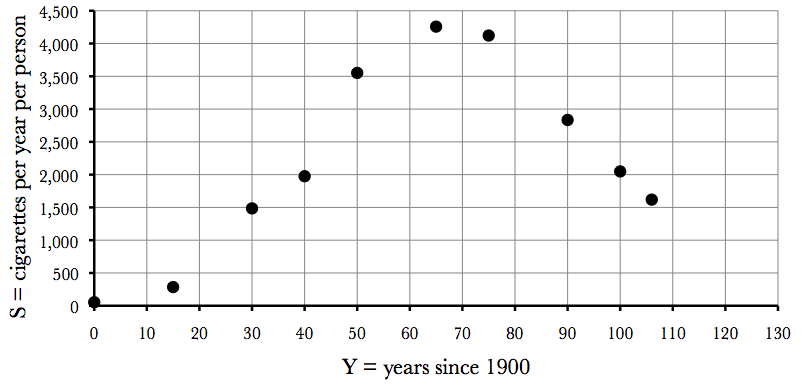
\includegraphics [width = 6in] {CigScatter3.png}}
%\end{center}

%Quick recap.  There are four key steps in drawing a graph by hand.

%\begin{enumerate}
%\item \textbf{Label} the axes.
%\item \textbf{Scale} the axes.
%\item \textbf{Plot} the points.
%\item \textbf{Connect} the points smoothly.
%\end{enumerate}
%
%In 1930 we have $Y=30$ and $S=\text{1,485}$.  That $S$-value is almost equal to \text{1,500}.  We draw the point just a tiny bit below the gridline for \text{1,500}.  It's okay if the point you draw looks on that line, but officially it's a tiny bit below. 


\today
